% For building the DRAM structure figure
% #1 x, #2 y, #3 no
\newcommand\noctile[3]{
    \draw (#1,#2) node[circle, draw, thick, minimum size=1cm] (r#3) {R};
    \draw (0.7 + #1, -0.7 + #2) node[rectangle, draw, thick, dashed, minimum size=1.2cm, anchor=north west] (t#3) {\emph{Tile}};
    \draw (r#3.-45) edge[thick, dashed] (t#3.135);
}

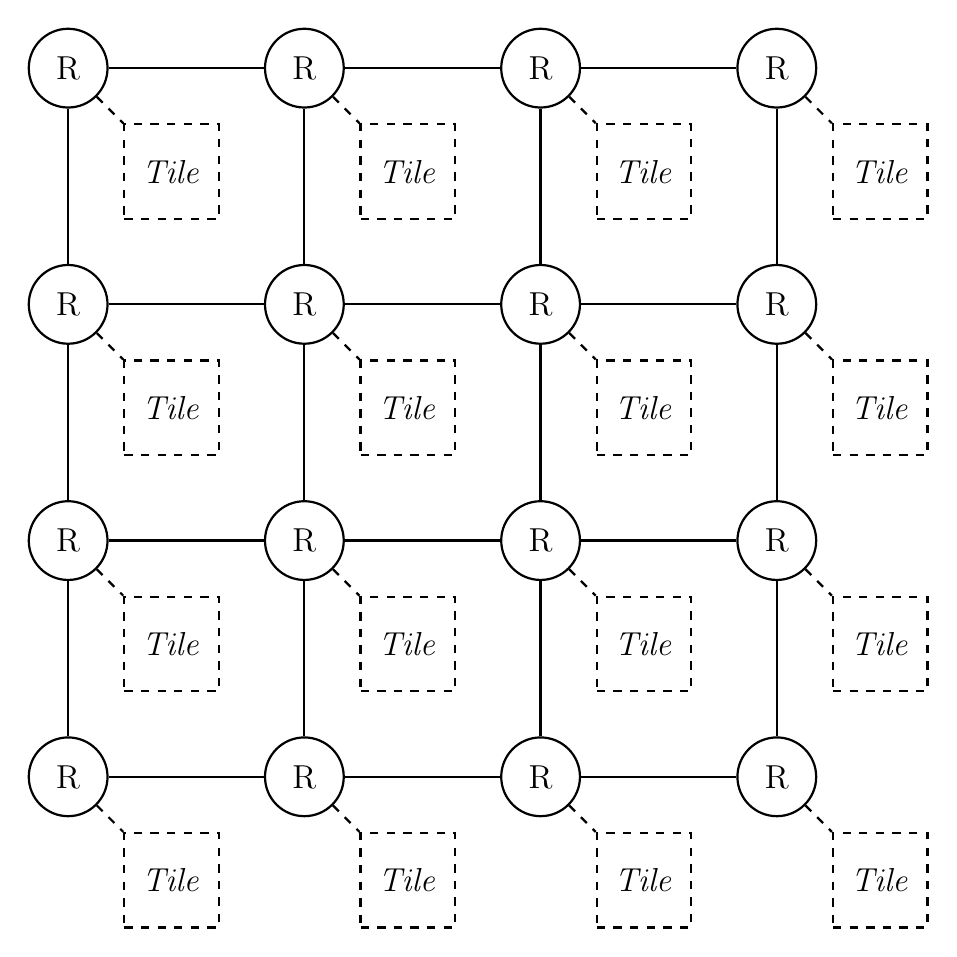
\begin{tikzpicture}[font={\fontsize{12pt}{12}\selectfont}]

\noctile{0}{0}{1}
\noctile{0}{3}{2}
\noctile{0}{6}{3}
\noctile{0}{9}{4}
\noctile{3}{0}{5}
\noctile{3}{3}{6}
\noctile{3}{6}{7}
\noctile{3}{9}{8}
\noctile{6}{0}{9}
\noctile{6}{3}{10}
\noctile{6}{6}{11}
\noctile{6}{9}{12}
\noctile{9}{0}{13}
\noctile{9}{3}{14}
\noctile{9}{6}{15}
\noctile{9}{9}{16}

\draw (r1.east) edge[thick] (r5.west);
\draw (r2.east) edge[thick] (r6.west);
\draw (r3.east) edge[thick] (r7.west);
\draw (r4.east) edge[thick] (r8.west);
\draw (r5.east) edge[thick] (r9.west);
\draw (r6.east) edge[thick] (r10.west);
\draw (r7.east) edge[thick] (r11.west);
\draw (r8.east) edge[thick] (r12.west);
\draw (r9.east) edge[thick] (r13.west);
\draw (r10.east) edge[thick] (r14.west);
\draw (r11.east) edge[thick] (r15.west);
\draw (r12.east) edge[thick] (r16.west);

\draw (r1.north) edge[thick] (r2.south);
\draw (r2.north) edge[thick] (r3.south);
\draw (r3.north) edge[thick] (r4.south);
\draw (r5.north) edge[thick] (r6.south);
\draw (r6.north) edge[thick] (r7.south);
\draw (r7.north) edge[thick] (r8.south);
\draw (r9.north) edge[thick] (r10.south);
\draw (r10.north) edge[thick] (r11.south);
\draw (r11.north) edge[thick] (r12.south);
\draw (r13.north) edge[thick] (r14.south);
\draw (r14.north) edge[thick] (r15.south);
\draw (r15.north) edge[thick] (r16.south);

\end{tikzpicture}
